%!TEX root = ../dissertation.tex
\chapter{Industrial Use Case}
\label{industrial-use-case}

In this chapter it will be presented a use case for the developed sentiment analysis model. For an initial test, have been crawled new data focused on the target subject, and after been processed for the sentiment classification, they have been presented with the Oracle Data Visualization Desktop tool. In the following paragraphs it will be discussed all the followed steps, and finally some information that have been extracted from the data.

\section{New Data Gathering}

For a preliminary use case of the sentiment analysis classification model discussed so far, it has been decided to introduce new information reputed useful for marketing analyses, with respect to the ones discussed for the already gathered dataset. The whole information downloaded in the new crawling were:
\begin{itemize}
	\item Forum's name;
	\item URL;
	\item Thread's title;
	\item Comment's timestamp;
	\item User's total number of comments;
	\item User's subscription date;
	\item Text;
	\item Quote.
\end{itemize}

The procedure was the same followed for the gathering of the training dataset. However, for this purpose, the only comments that matter are the ones with a reference to the brand Porsche, so only comments belonging to Porsche's discussions were crawled. For future works, comments are supposed to be crawled from every kind of discussion, detecting automatically the pertinence to the target brand.\\
Some basic statistics about crawled comments are shown in Figure \ref{table:new-comments-test}.

\begin{table}[H]
	\centering
	\begin{tabular}{ | c | c | c | } 
		\hline
		\textbf{Forum} & \textbf{\# Threads} & \textbf{\# Comments}\\
		\hline
		Quattroruote & 12 & 473 \\
		\hline
		Bmwpassion & 8 & 883 \\
		\hline
		Porschemania & 37 & 5,039 \\
		\hline
		\hline
		TOTAL & 57 & 6,395 \\
		\hline		
	\end{tabular}
	\caption{Distribution of new comments.}
	\label{table:new-comments-test}
\end{table}

The threads have been manually selected. Have been chosen the most discussed threads, including also the main discussions related to a car model. All the comments have been classified by the sentiment analysis classifiers, with respect to the "engine", "brand", "exteriors" and "support" topics. Naturally, since data have not been manually labeled, it is not possible to evaluate scores about the quality of the classification, but the only way to achieve it, is looking at the details of the comments, like in a real world application.\\
In the following paragraph it will show how data have been visualized, exploiting a powerful data visualization tool.


\section{Data Visualization}

Data visualization consists on graphical representation of the data. It is used to visualize relationships between the data, in order to communicate results to the stakeholders, that eventually use the data for diverse purposes, such as for making marketing choices. For visualize the ultimate data that have been collected and classified, it has been utilize Oracle Data Visualization Desktop (\url{https://www.oracle.com/middleware/technologies/oracle-data-visualization-desktop.html}), that is a useful tool that permit with a simple interface to manage data flows and explore data from local or remote origins.\\
In the next paragraphs it will be presented some information about the brand Porsche, that have been extracted from new collected and annotated data.


\subsection{Preliminary Information about Sentiment expressed in the Forums}

In Figure \ref{fig:preliminar-info} have been showed some simple statistics about the collected data.

\begin{figure}[H]
	\centering
	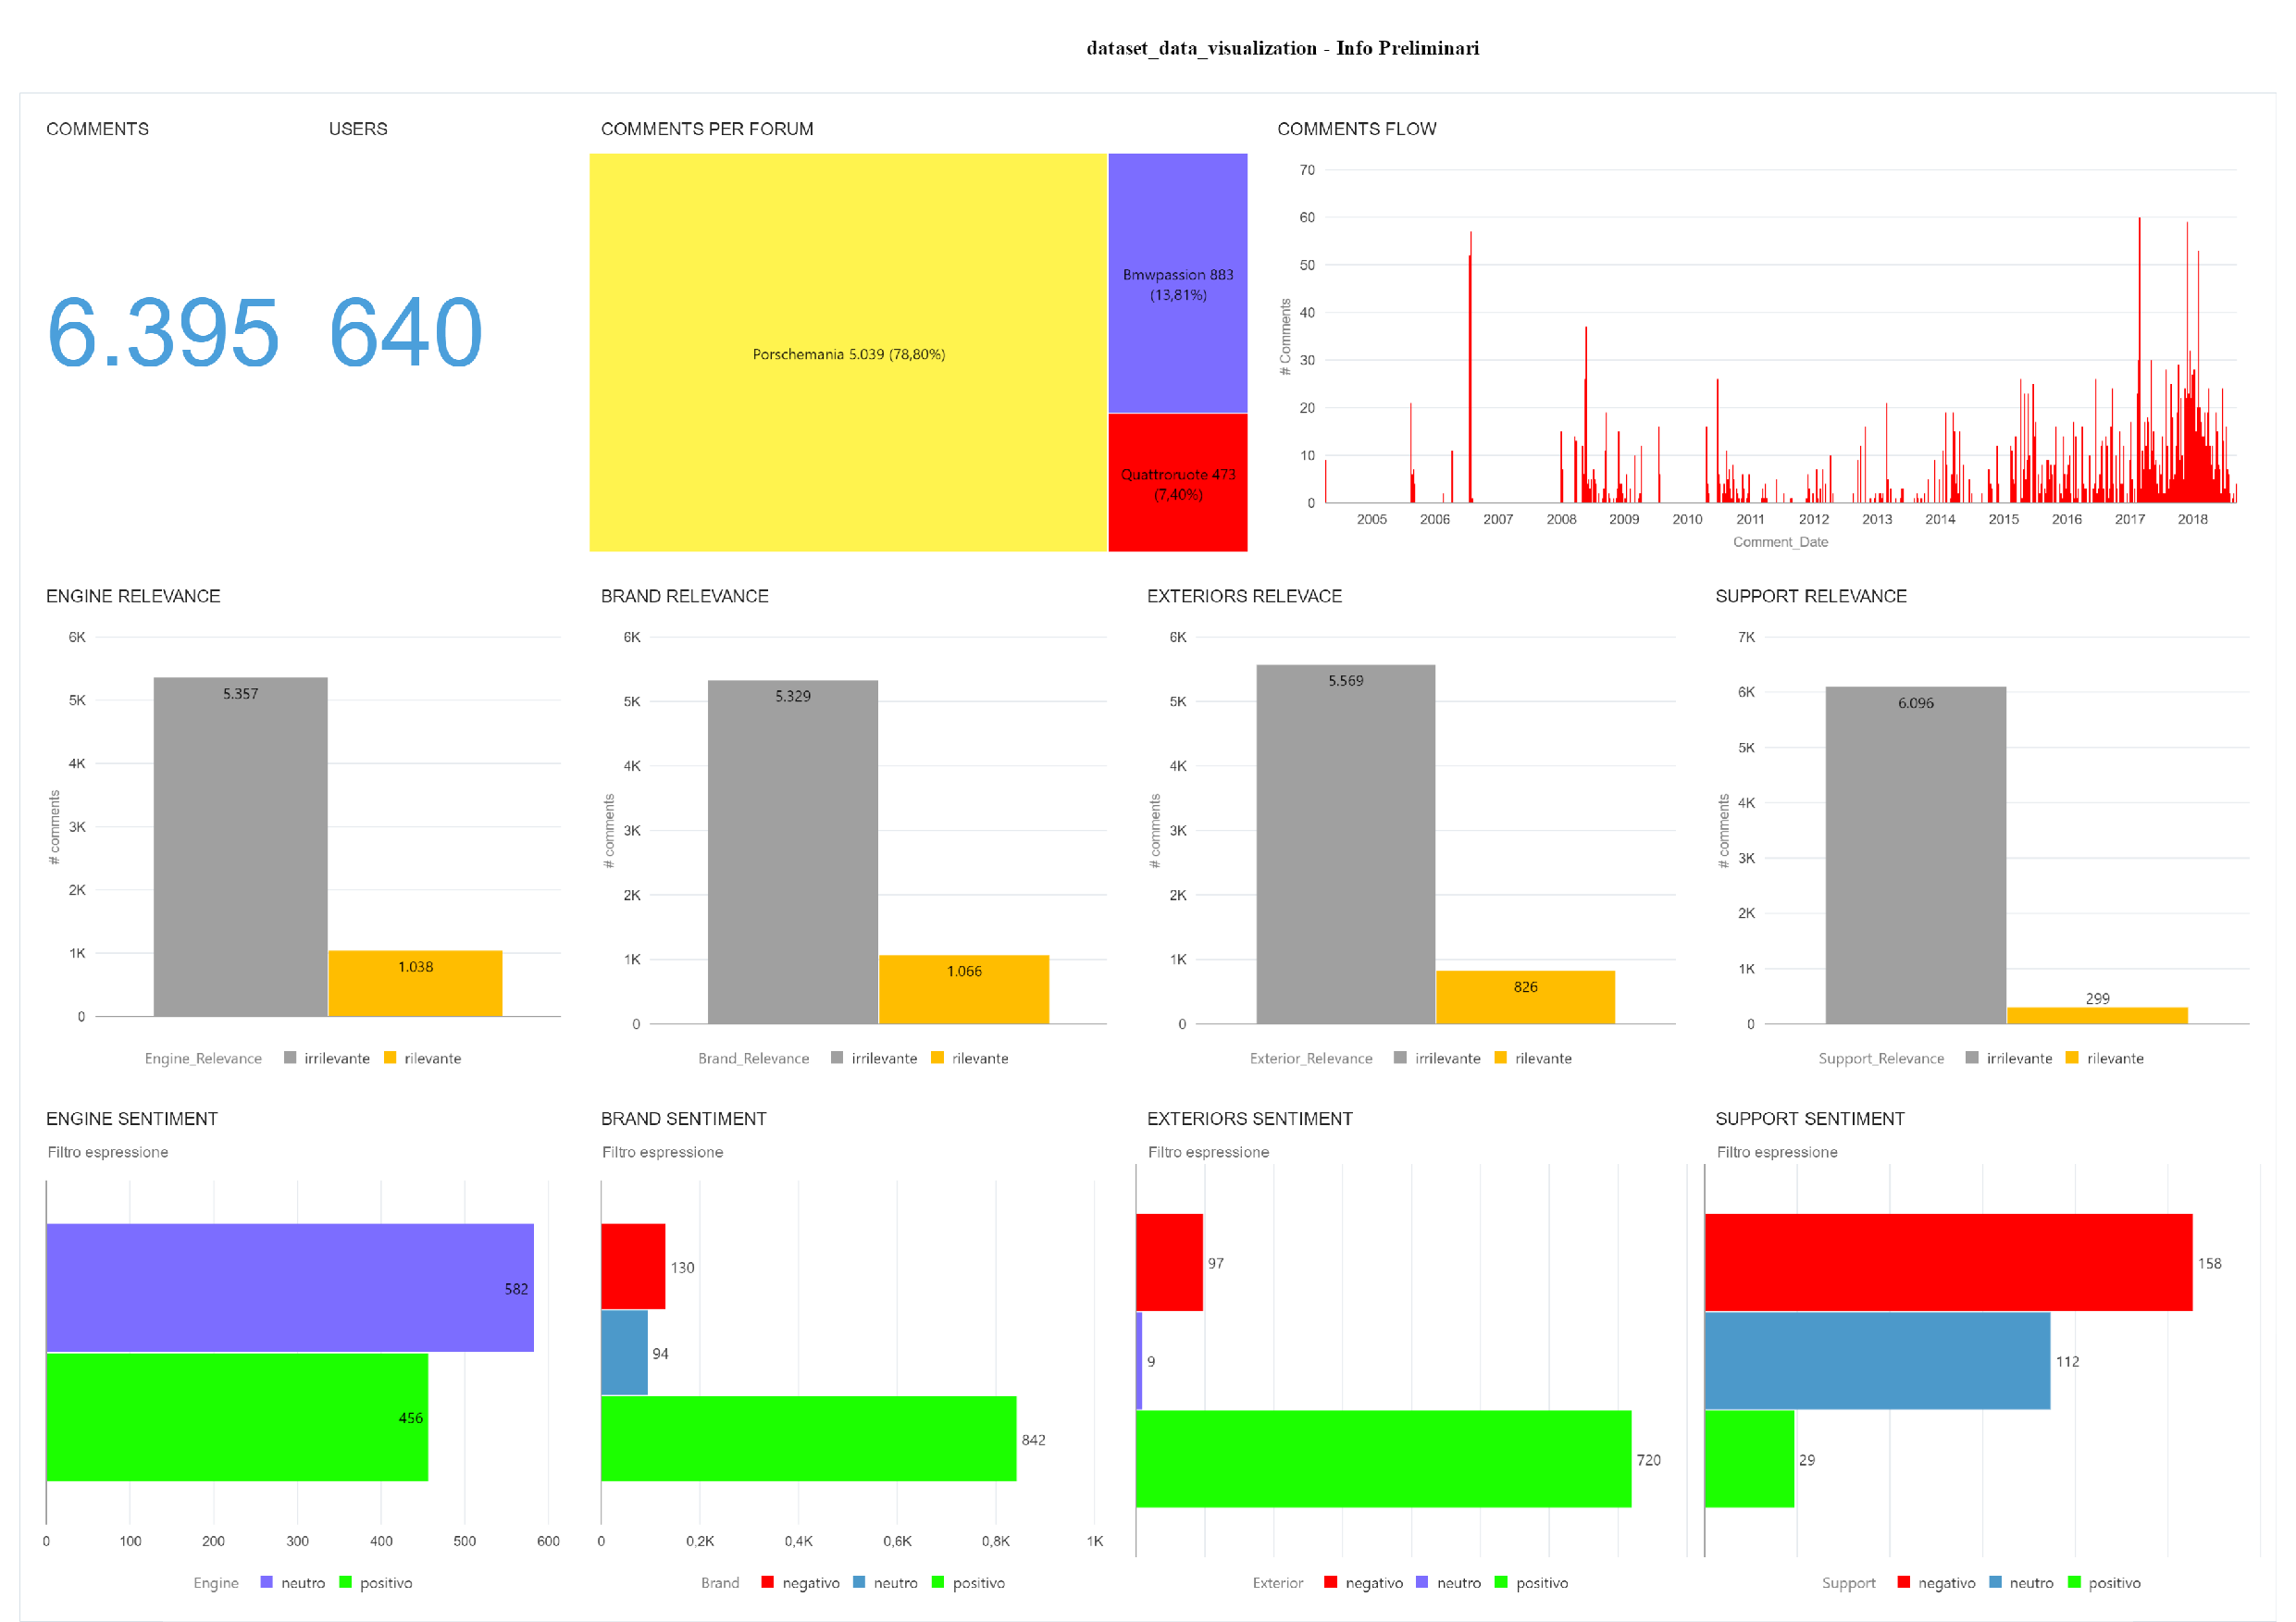
\includegraphics[width=\textwidth]{figures/odv_export/dataset_data_visualization_1.pdf}
	\caption{Overall statistics about the sentiment.}
	\label{fig:preliminar-info}
\end{figure}

It is easily shown the number of new gathered comments, and the total number of different users. Comments are distributed with high frequency on last years mostly because selected threads are referred to ultimate car models, and so are the relative discussions. From the last graphics it is possible to deduce some expected relevance, and some surprisingly others. Starting from the class "engine", it is a good result for the brand, especially for a sporty one such as Porsche, because in shows the customers' satisfaction about this particular topic. At contrary, comments about "support" show an imbalance to the negative sentiment, that is expected, since in these comments usually the main argument is some breaks or situation where the customer care was not actually good.


\subsection{Sentiment Information about Porsche Panamera model}

In Figure \ref{fig:panamera-snt} is have been shown some sentiment information about the Porsche Panamera model. The filter on the car model was made looking for key-words, so it is not sophisticated, in fact it will be one of the main enhancements to do for this work. It is interesting to see that comments' flow reached some peaks around years 2009 and last years, that coincides with the first presentation of the model in the 2009, and the newer model in 2016.

\begin{figure}[H]
	\centering
	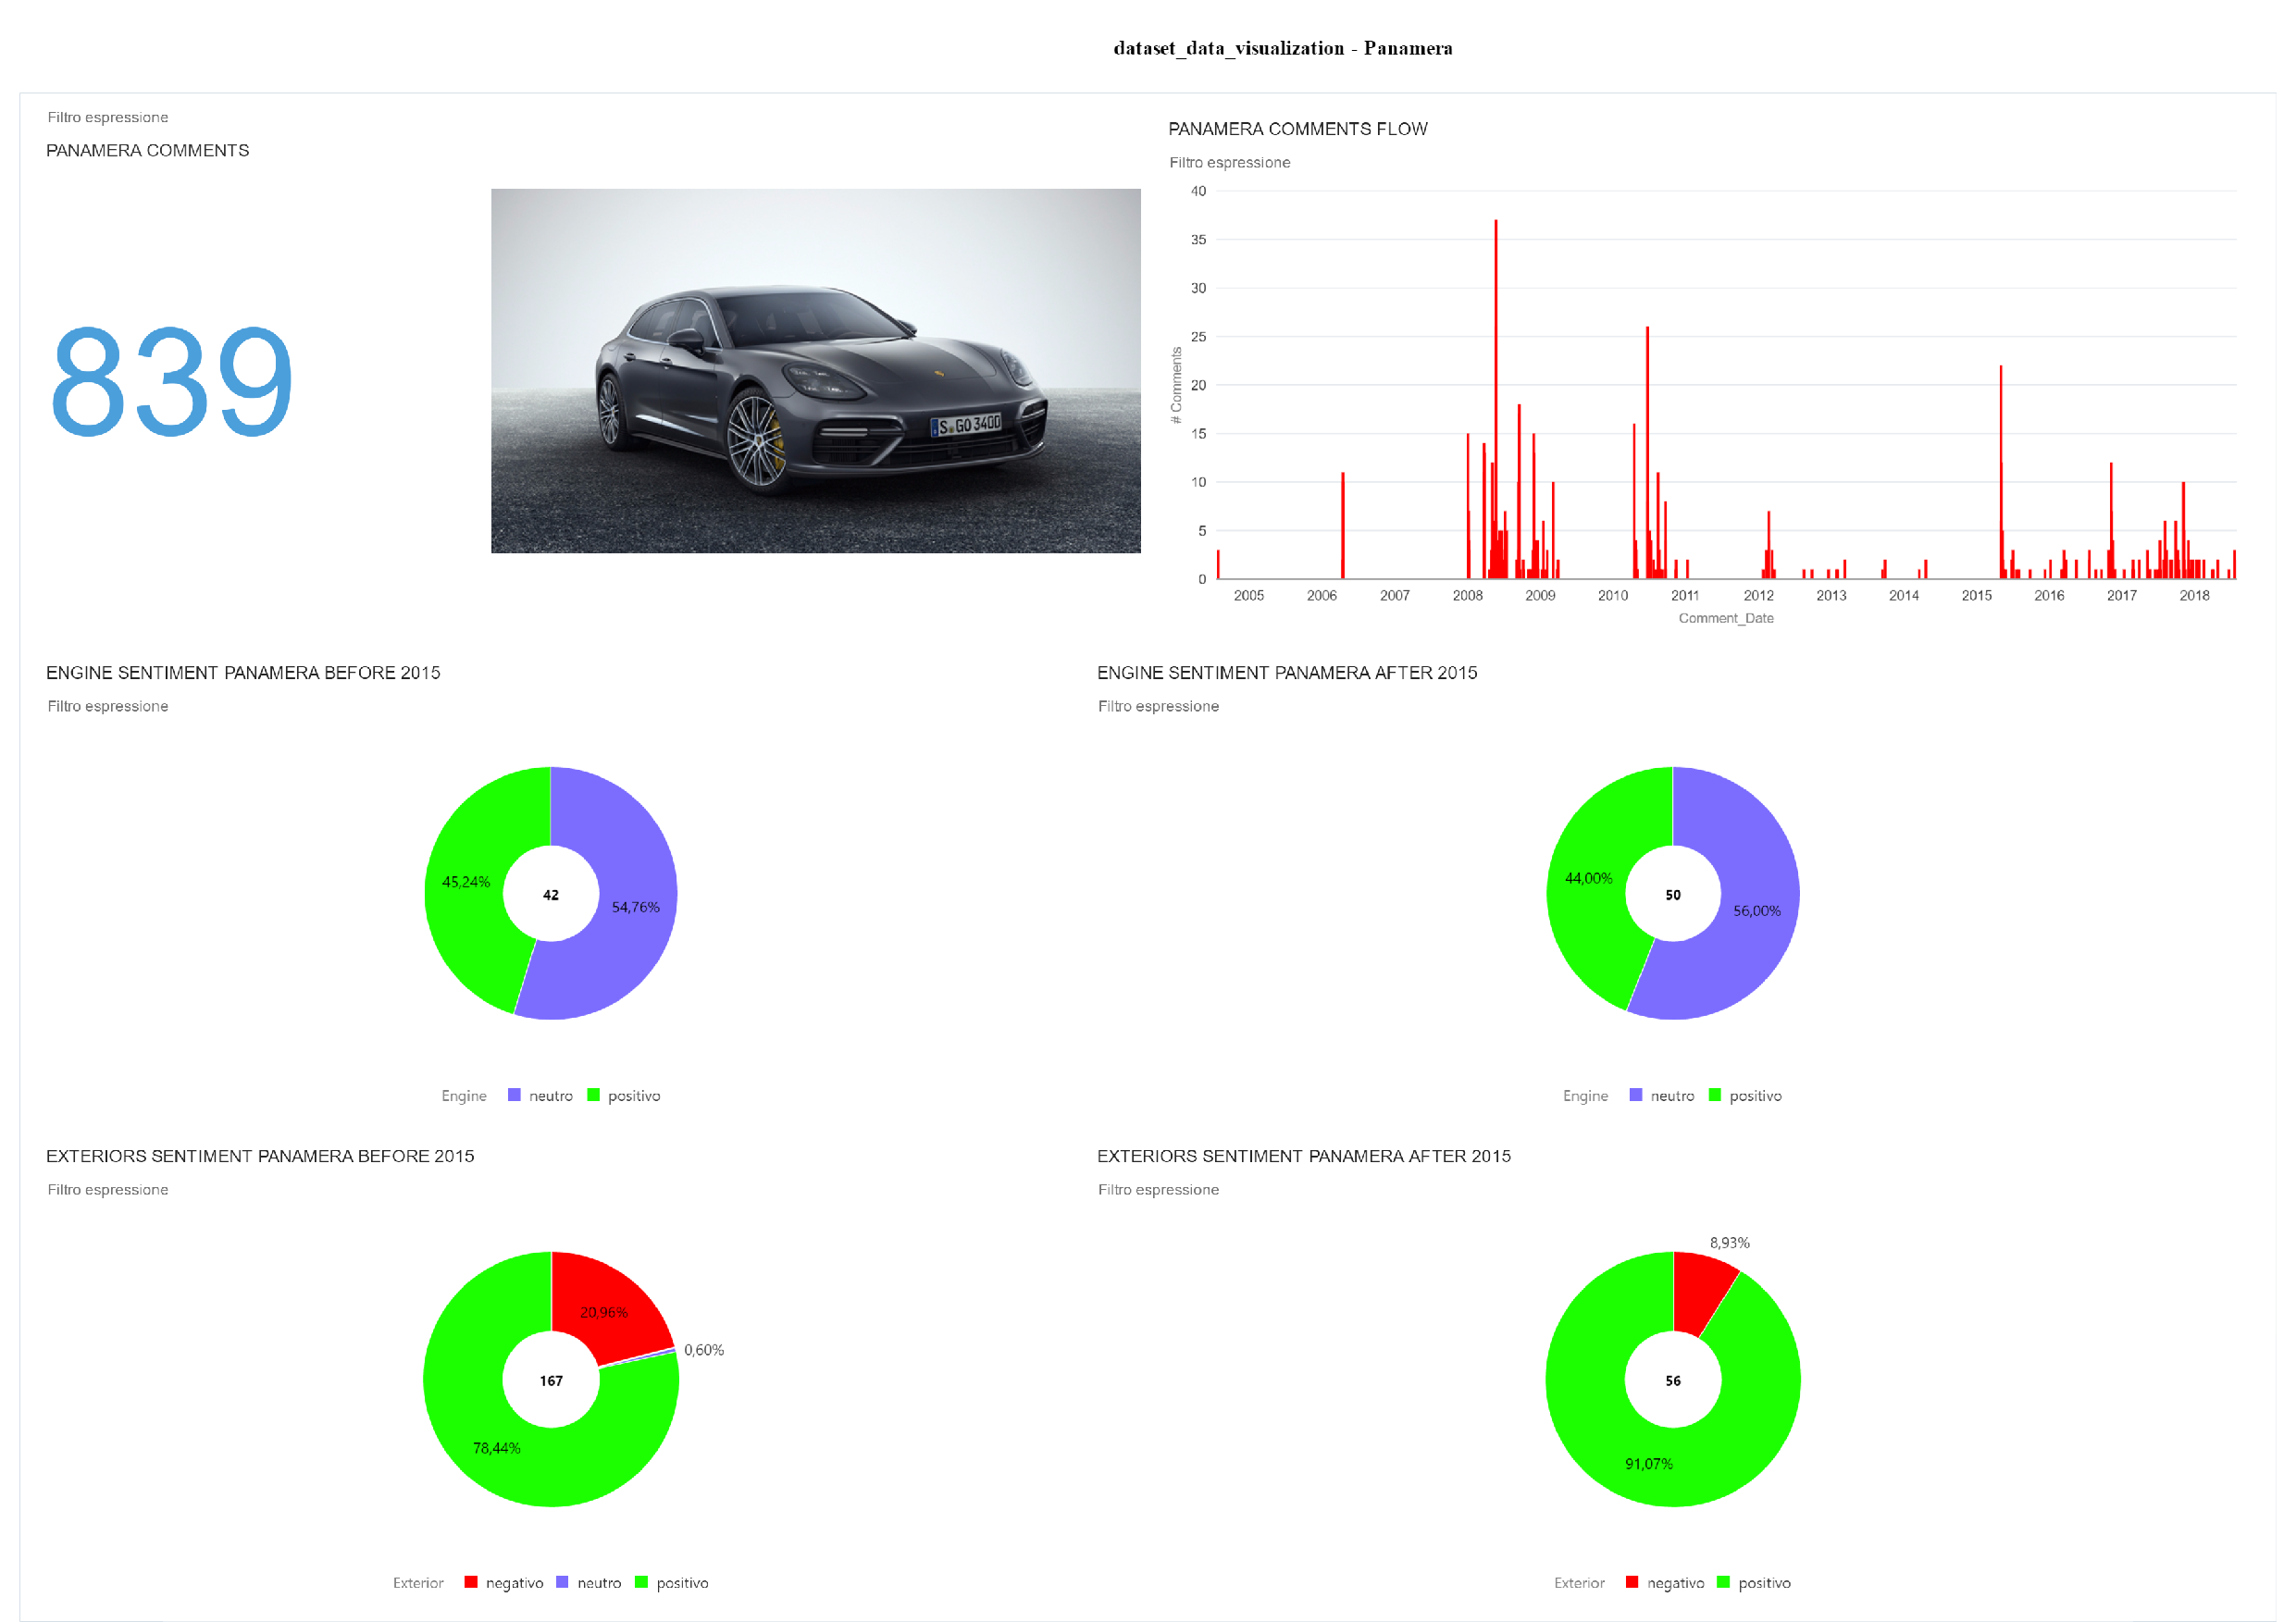
\includegraphics[width=\textwidth]{figures/odv_export/dataset_data_visualization_2.pdf}
	\caption{Sentiment polarities about Panamera model.}
	\label{fig:panamera-snt}
\end{figure}

For this car model it will be interesting to see how sentiment changed across the two versions. It has been chosen the separating year as 2015, and it was evaluate the sentiment about "engine" and "exteriors" before and after that year. The data show unchanged polarity about the engine, and a little improvement on exteriors, which is a good news since it was a very discussed model especially for its exteriors.



\subsection{Sentiment Information about Porsche 911 (version 992) model}

The same analysis has been made for the 992 model, which is the newer version of the famous 911. In Figure \ref{fig:992-snt} have been shown some statistics. Comments' flow has been made looking for mentions about just the 992 model, while below statistics are referred to the general 911 model.

\begin{figure}[H]
	\centering
	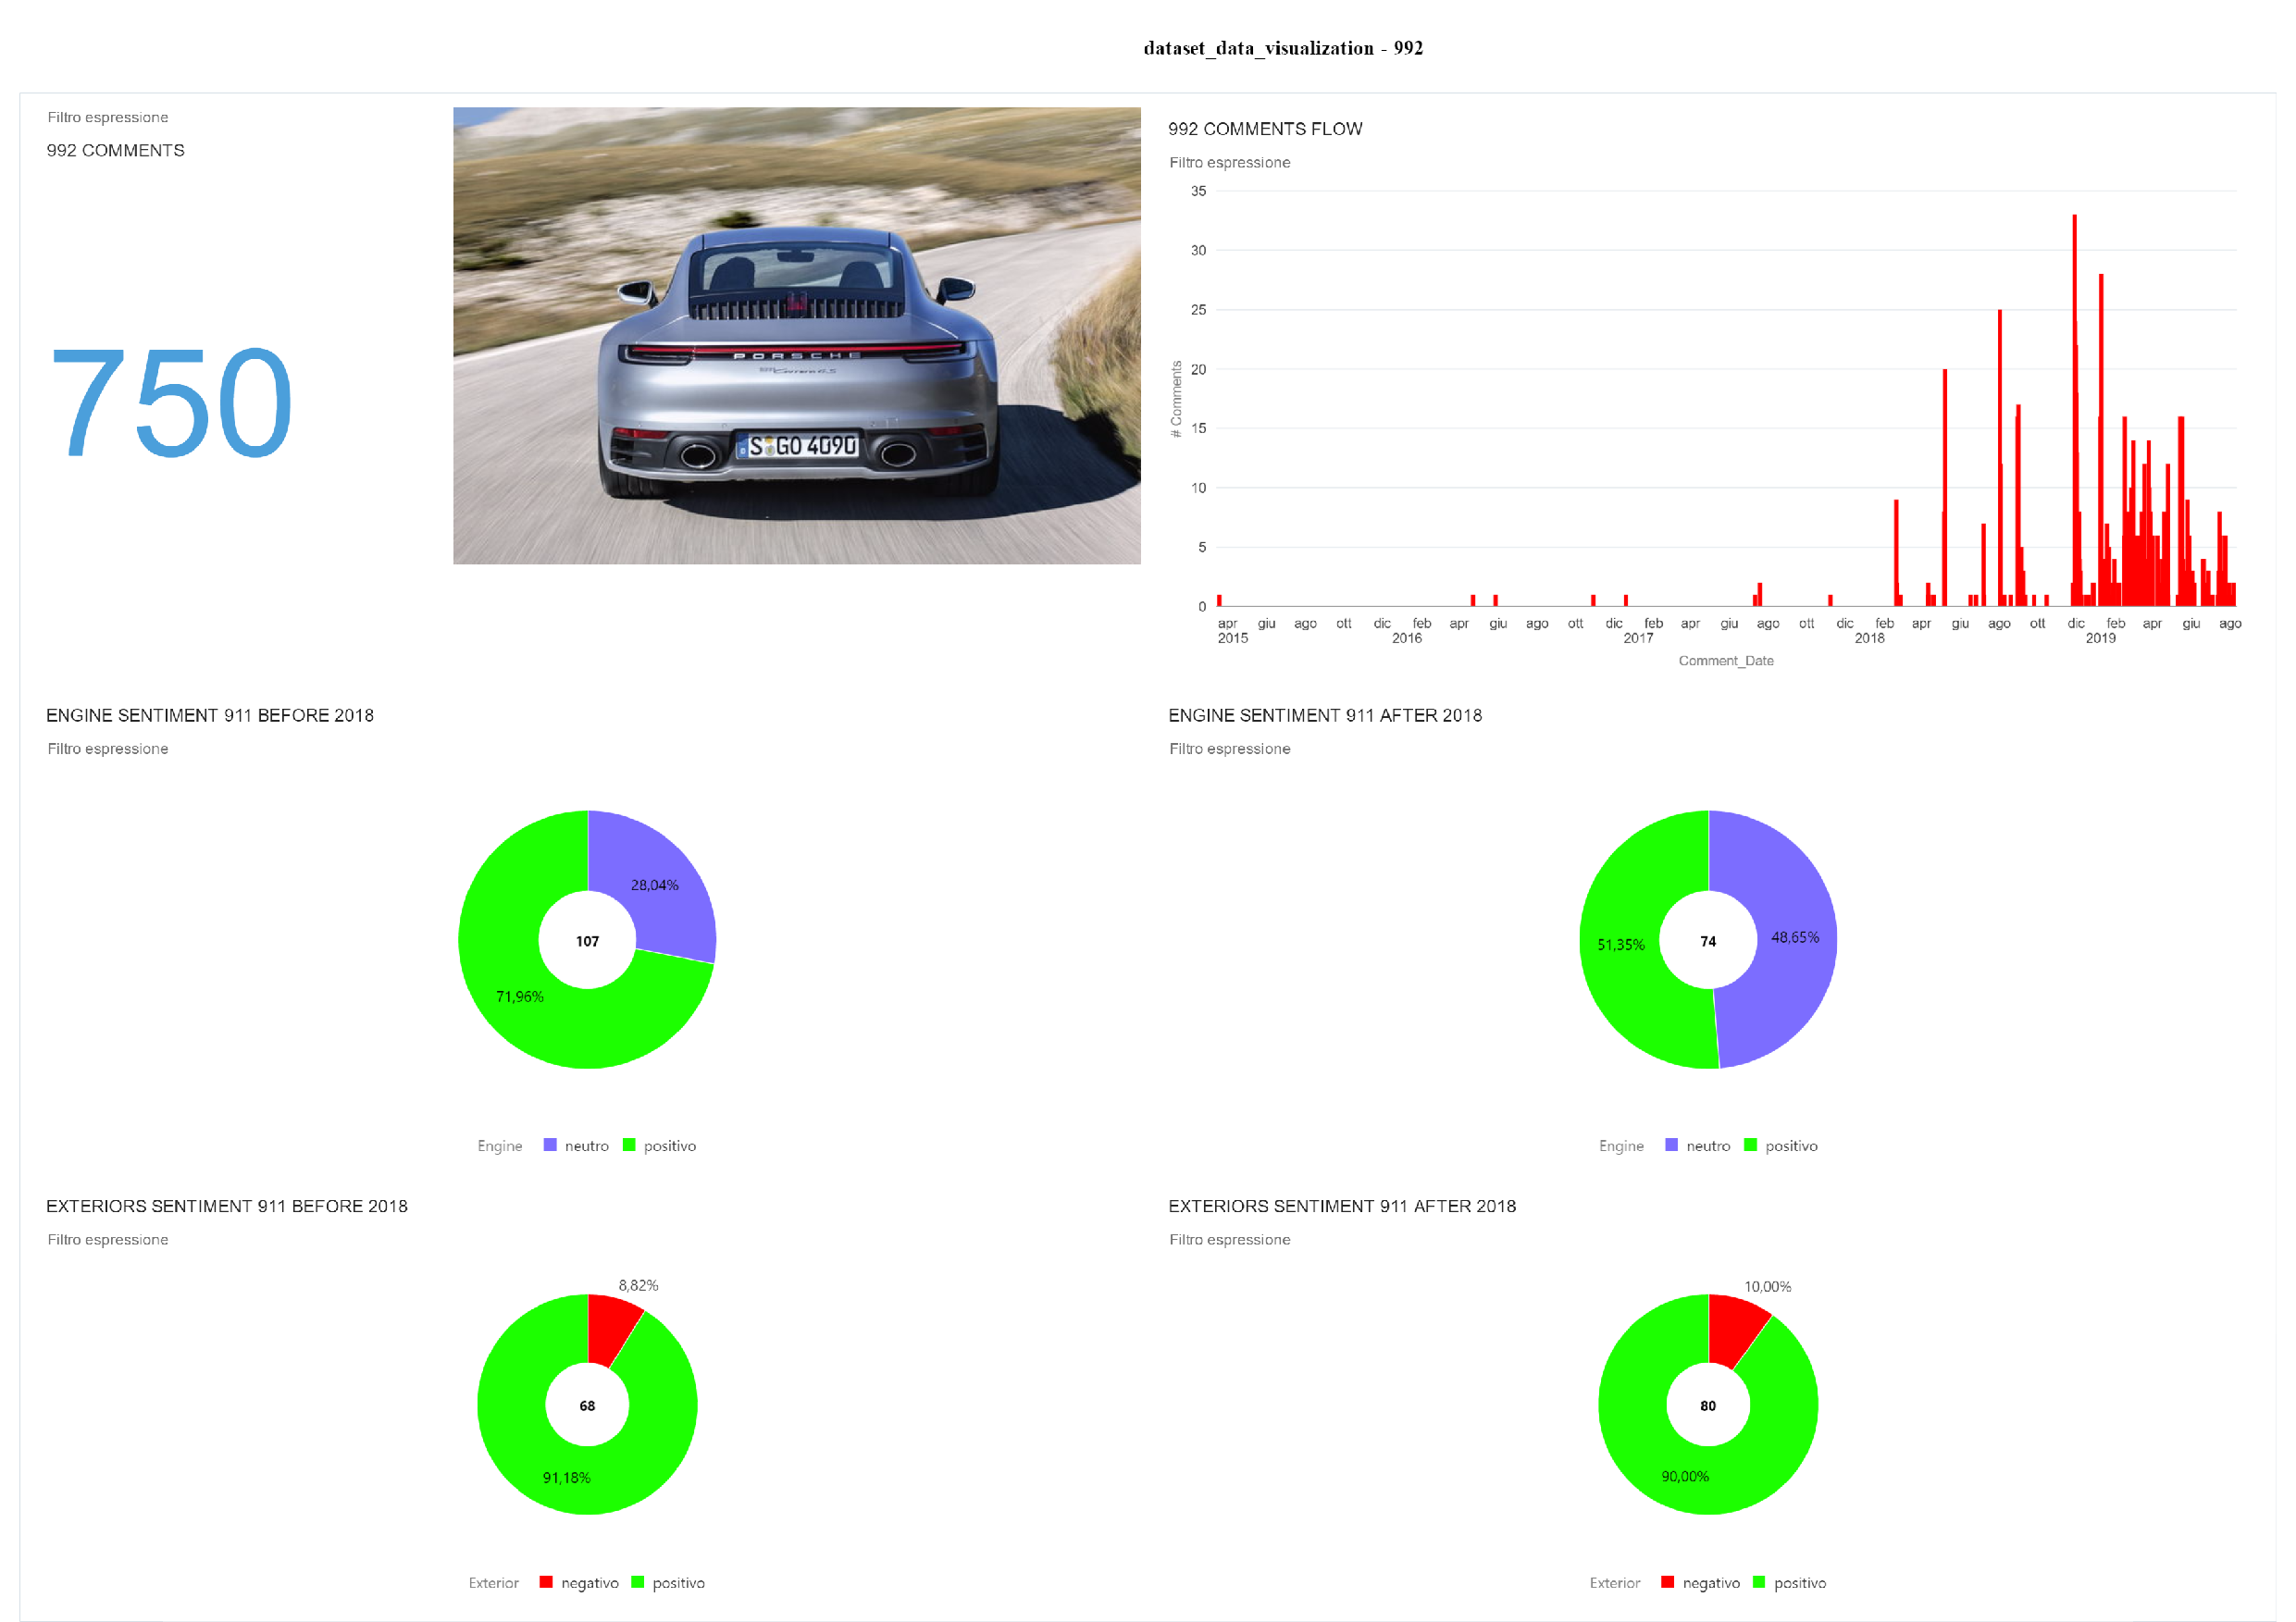
\includegraphics[width=\textwidth]{figures/odv_export/dataset_data_visualization_4.pdf}
	\caption{Sentiment polarities about 911 (992 version) model.}
	\label{fig:992-snt}
\end{figure}

As shown in the comments' flow, the car is mentioned just in these years, which is expected, since it is produced since 2019, but some leaks came in the earlier periods. Sentiments have been evaluated before and after the 2018, which has been considered the separating year for the older and the newer 911 model. The data show worse sentiment about the engine with a minor percentage of positive comments, but still not negative ones. At the same time, the trend about the exteriors remained the same, showing almost the same people's satisfaction about the style of the model.


\subsection{Sentiment Information about Cars' Exteriors}

In Figure \ref{fig:ext-year-snt} it has been shown the trend of sentiment polarity across years, for what concerns the models Panamera, 911 and 718. For this visualization, filtering has been made still with key-words, but just on comments and quotes.

\begin{figure}[H]
	\centering
	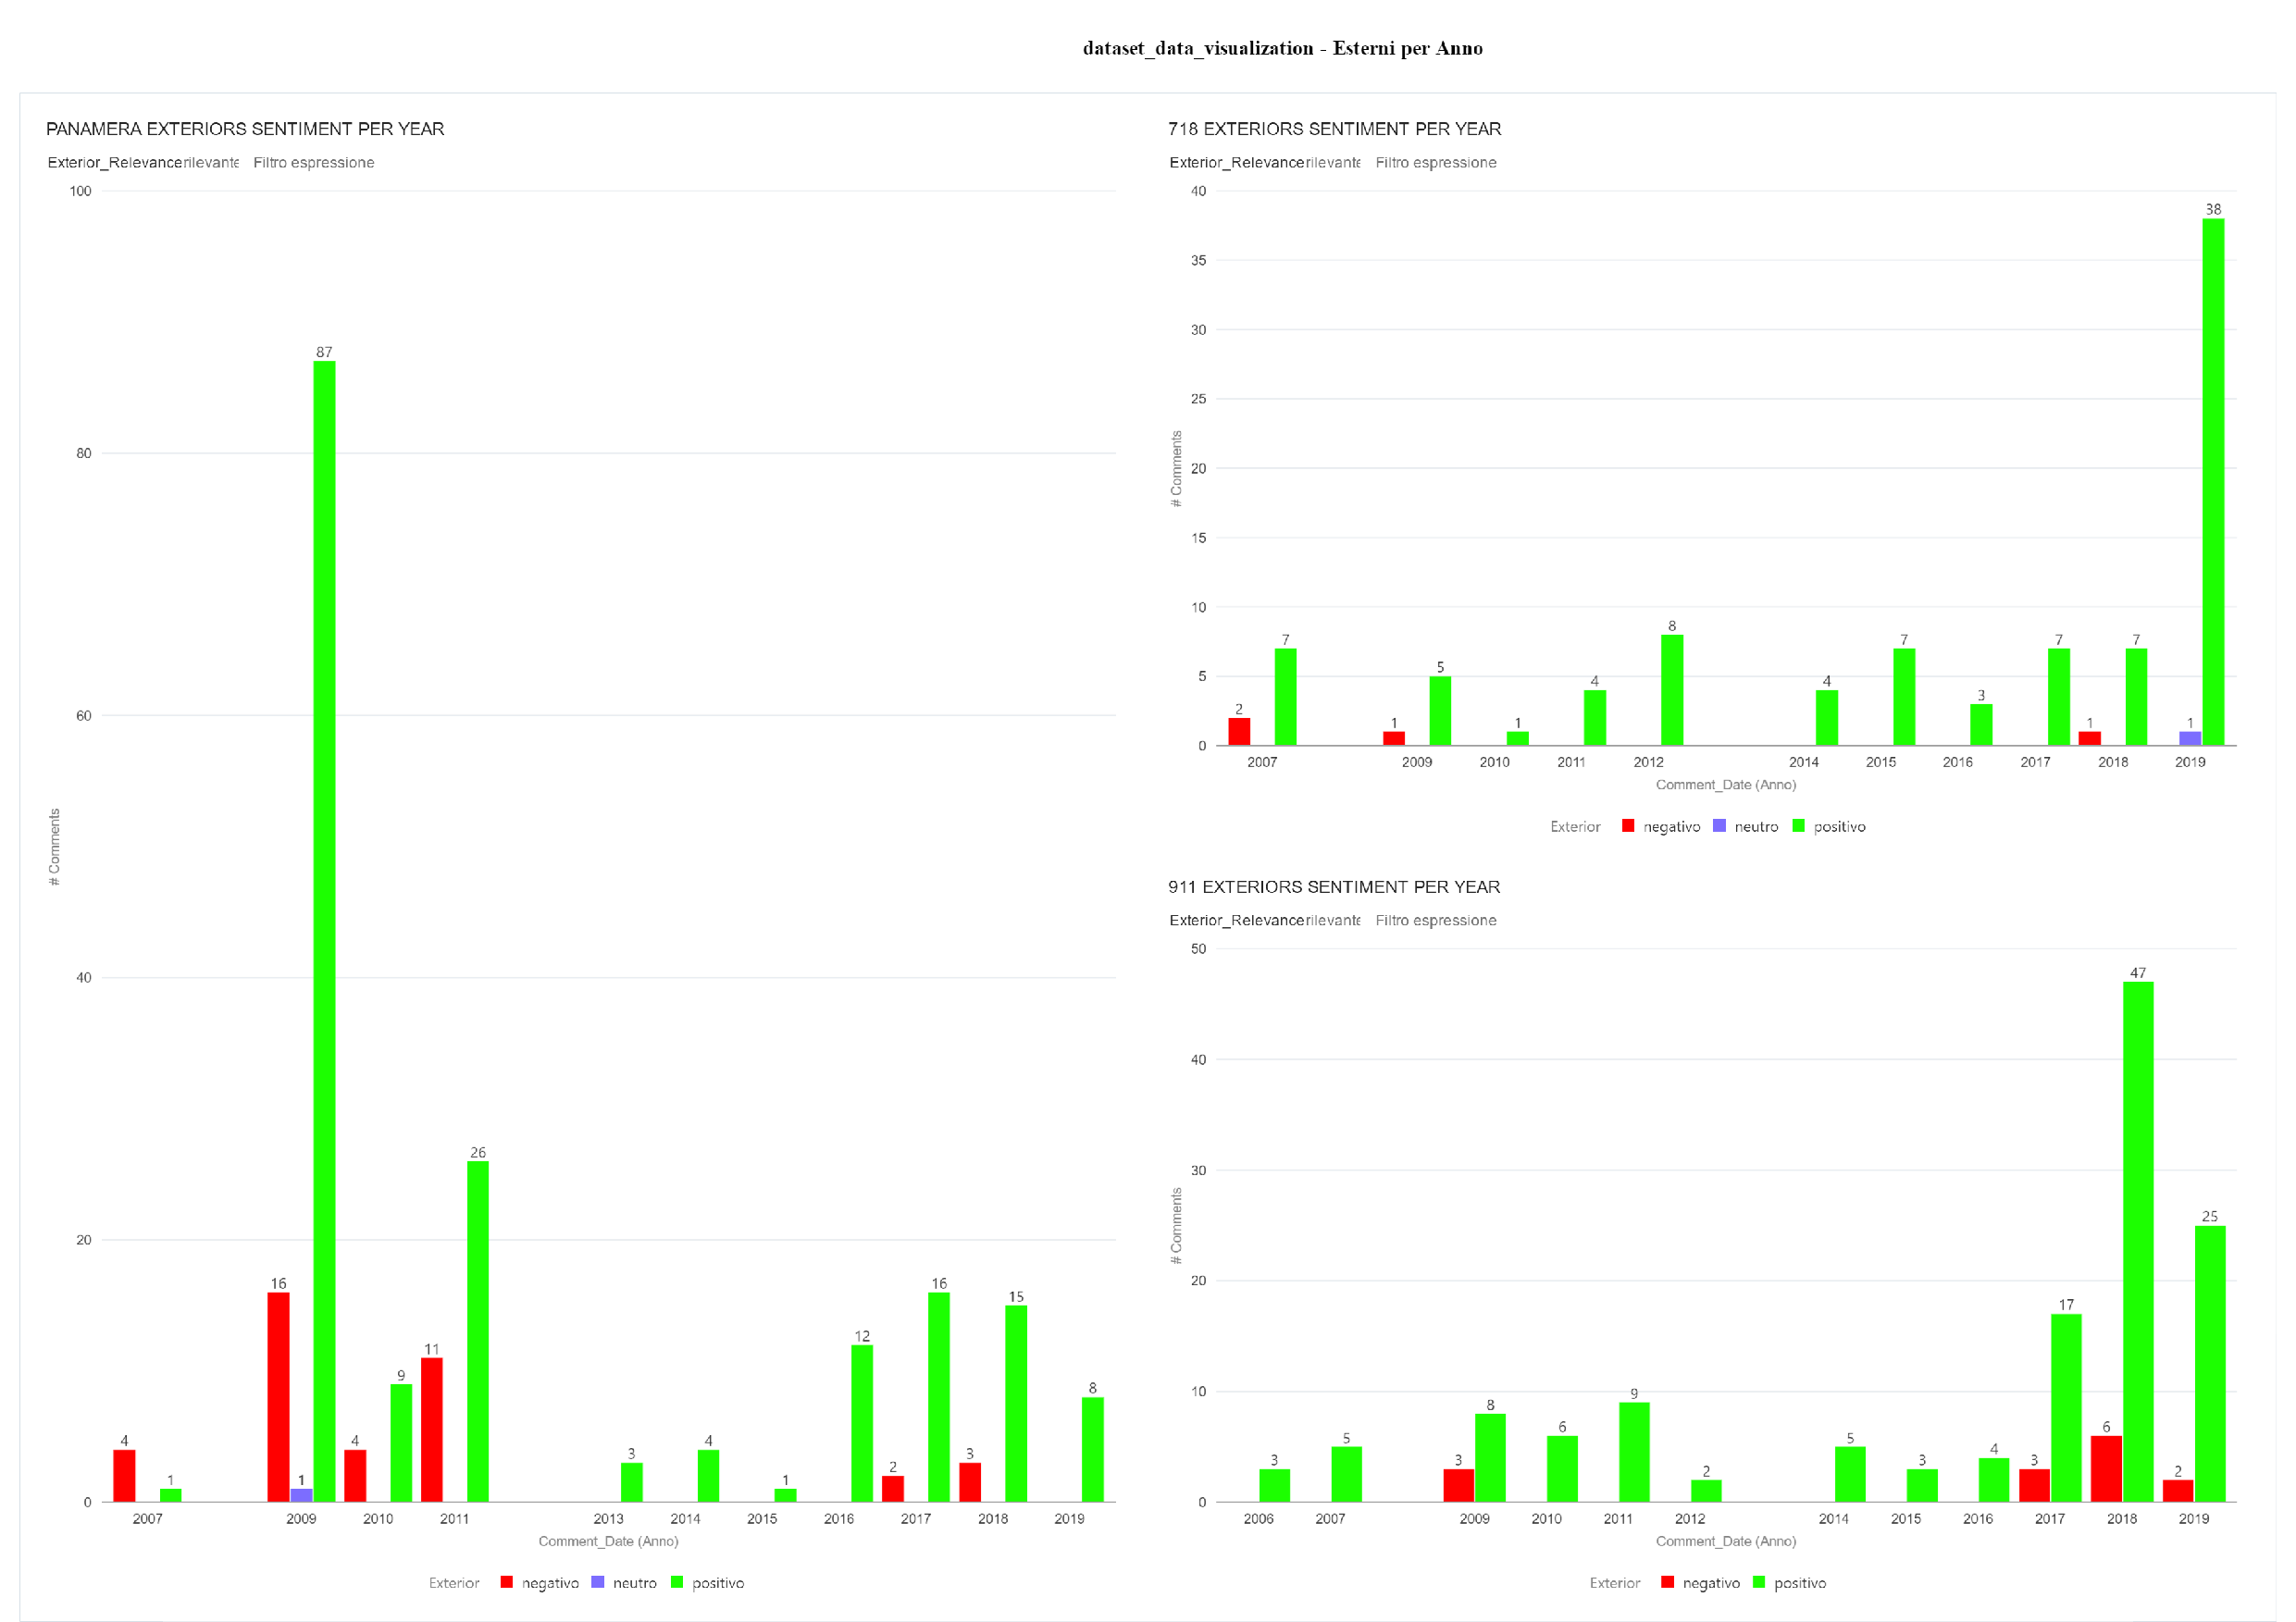
\includegraphics[width=\textwidth]{figures/odv_export/dataset_data_visualization_5.pdf}
	\caption{Sentiment polarities of some models on the years.}
	\label{fig:ext-year-snt}
\end{figure}

The main information that is possible to extract, regards the Panamera model, that again show improvements about its exteriors from the first model to the last one, while for the other models, no interesting information has been extracted.



\subsection{Trend of Comments with respect to Users' Seniority}

In Figure \ref{fig:model-senior} have been showed some information about users' seniority. Seniority has been calculated as the difference between comments' date and the users' subscription date.

\begin{figure}[H]
	\centering
	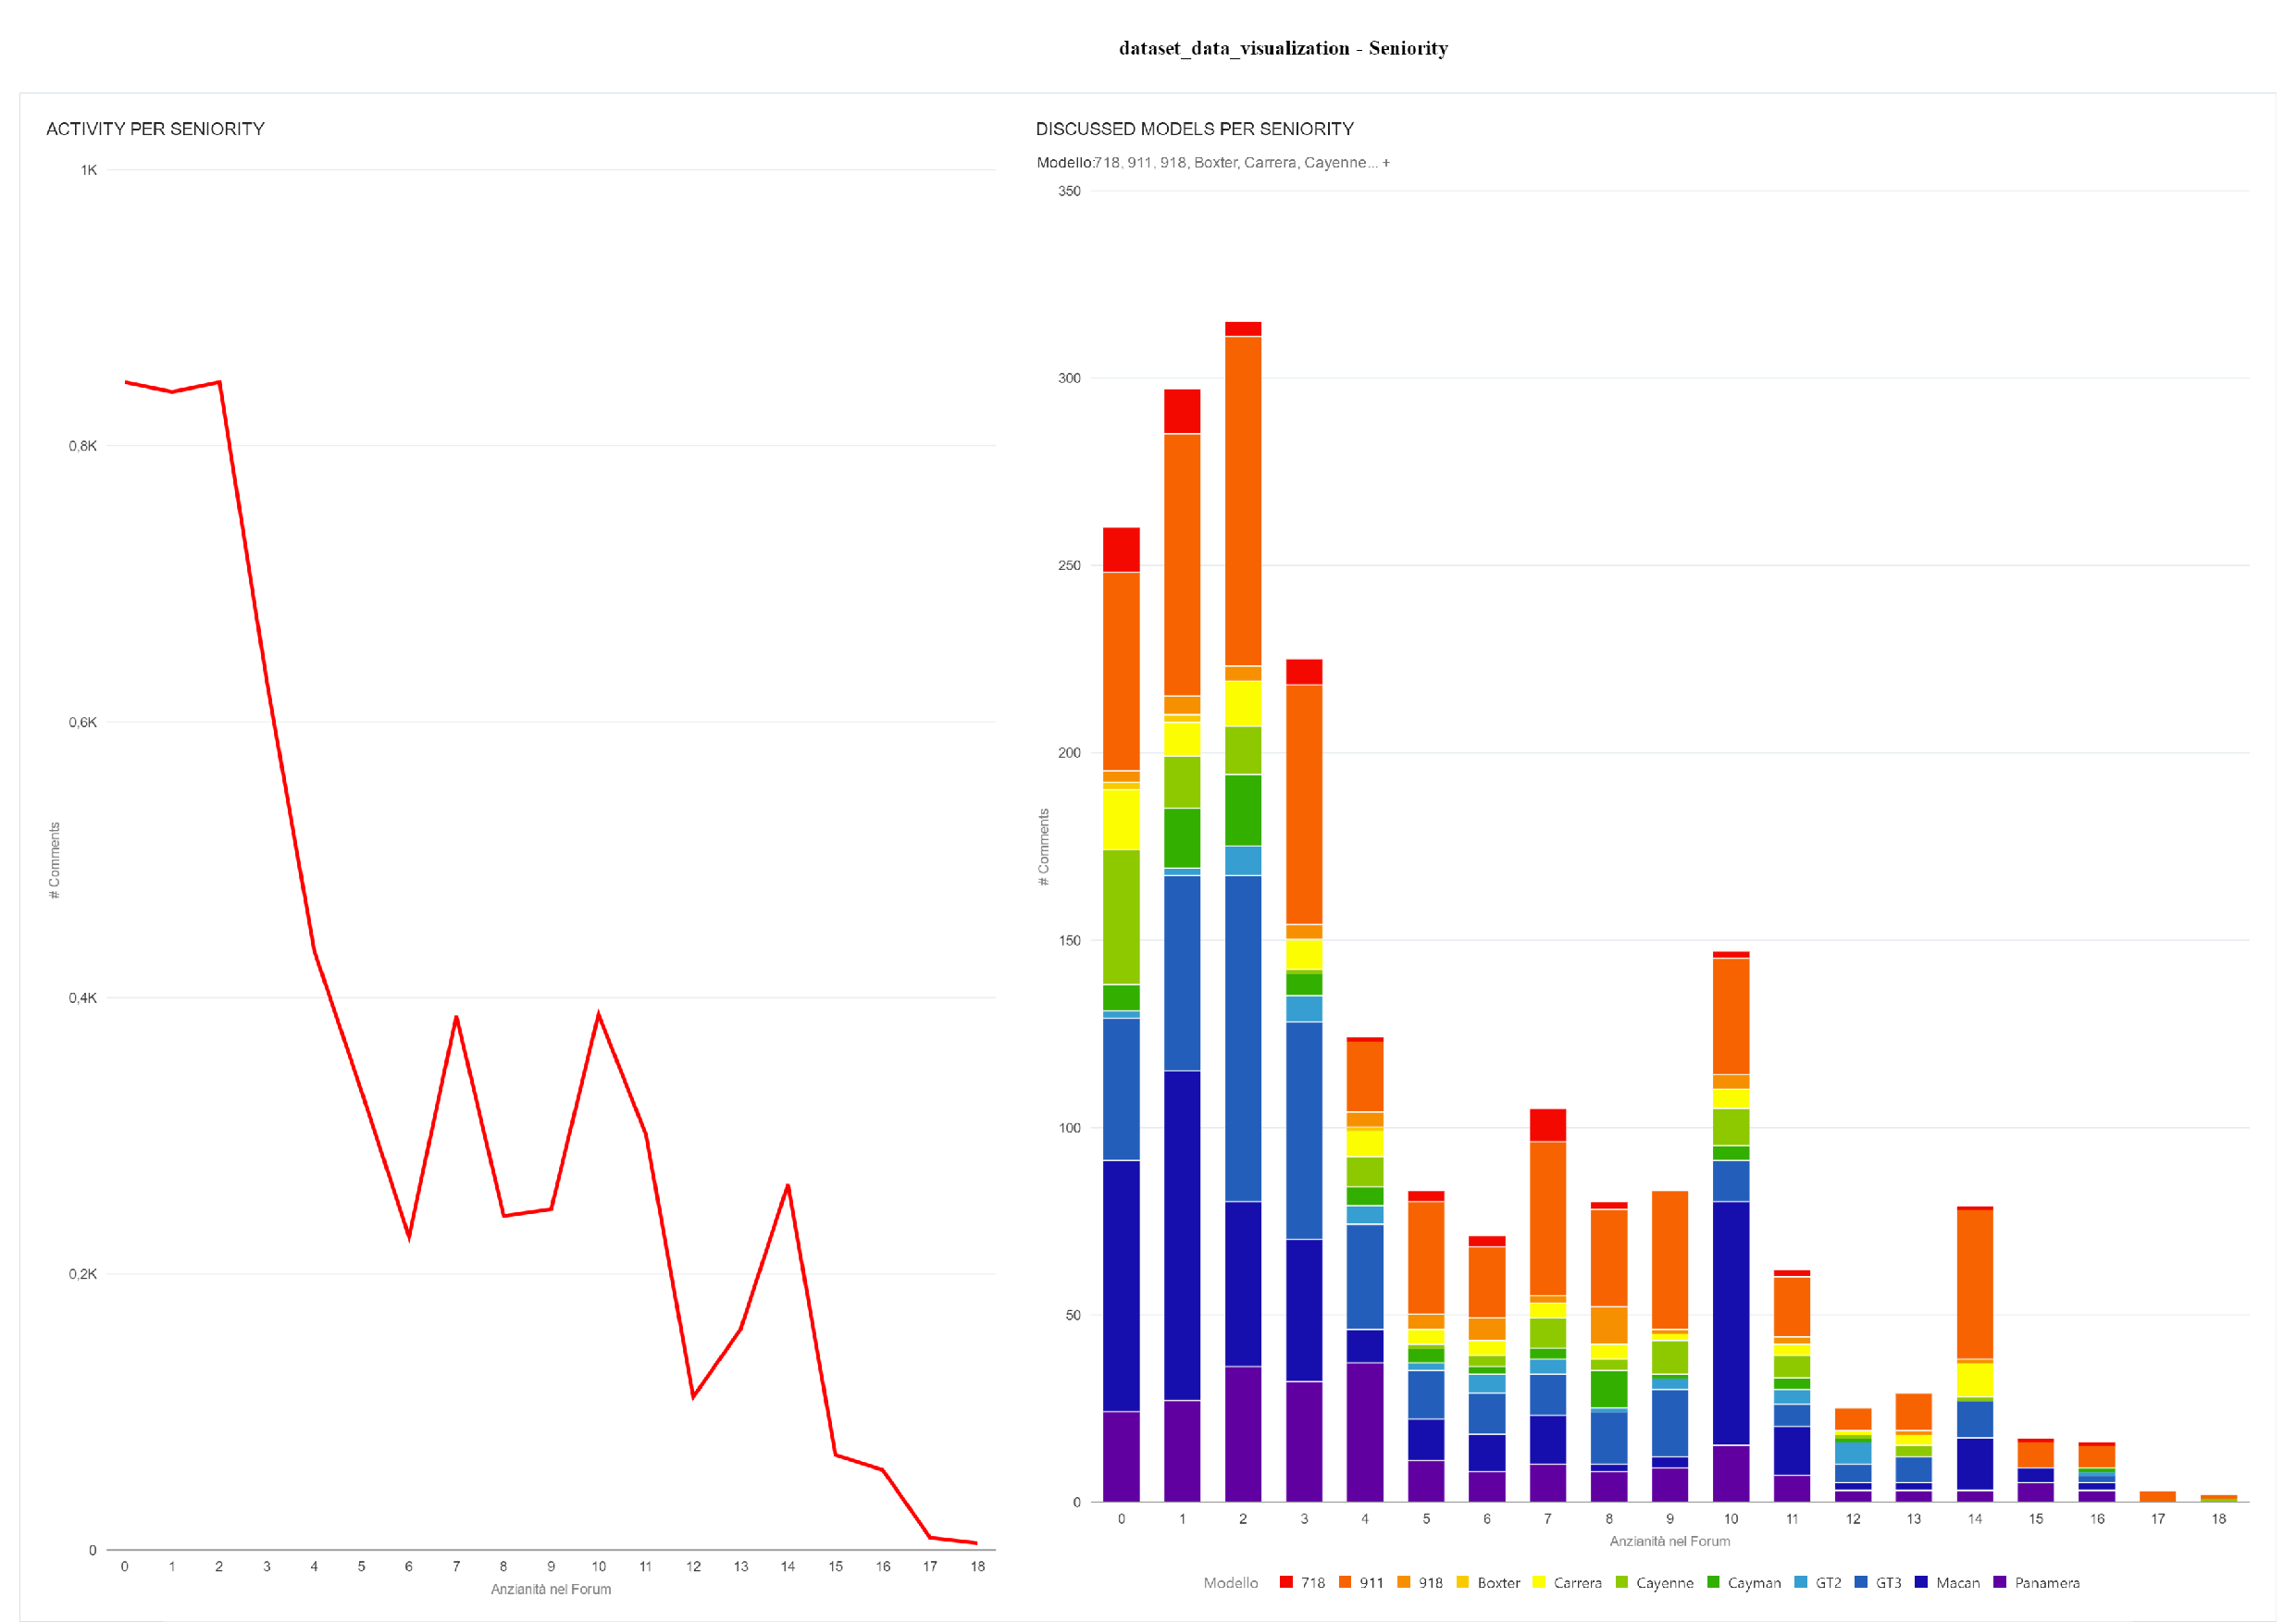
\includegraphics[width=\textwidth]{figures/odv_export/dataset_data_visualization_9.pdf}
	\caption{Models discussed per users' seniority.}
	\label{fig:model-senior}
\end{figure}

In the first graphic it is shown that users in general are very active in the earliest periods after the subscription, while the activity decreases on the increasing of the years after the subscription. It also has been shown the most discussed car modes with respect to the seniority, but it actually does not shown relevant information, but the fact that the most discussed ones remain actually the same.

\subsection{Most discussed Models}

In Figure \ref{fig:models} have been shown the most discussed models across the years. Models have been also divided in some sub-categories, for instance even if Boxter and Cayman are both belonging to the 718 family, they have been still separated. Obviously have been collected just the most relevant models, ignoring for instance older ones.

\begin{figure}[H]
	\centering
	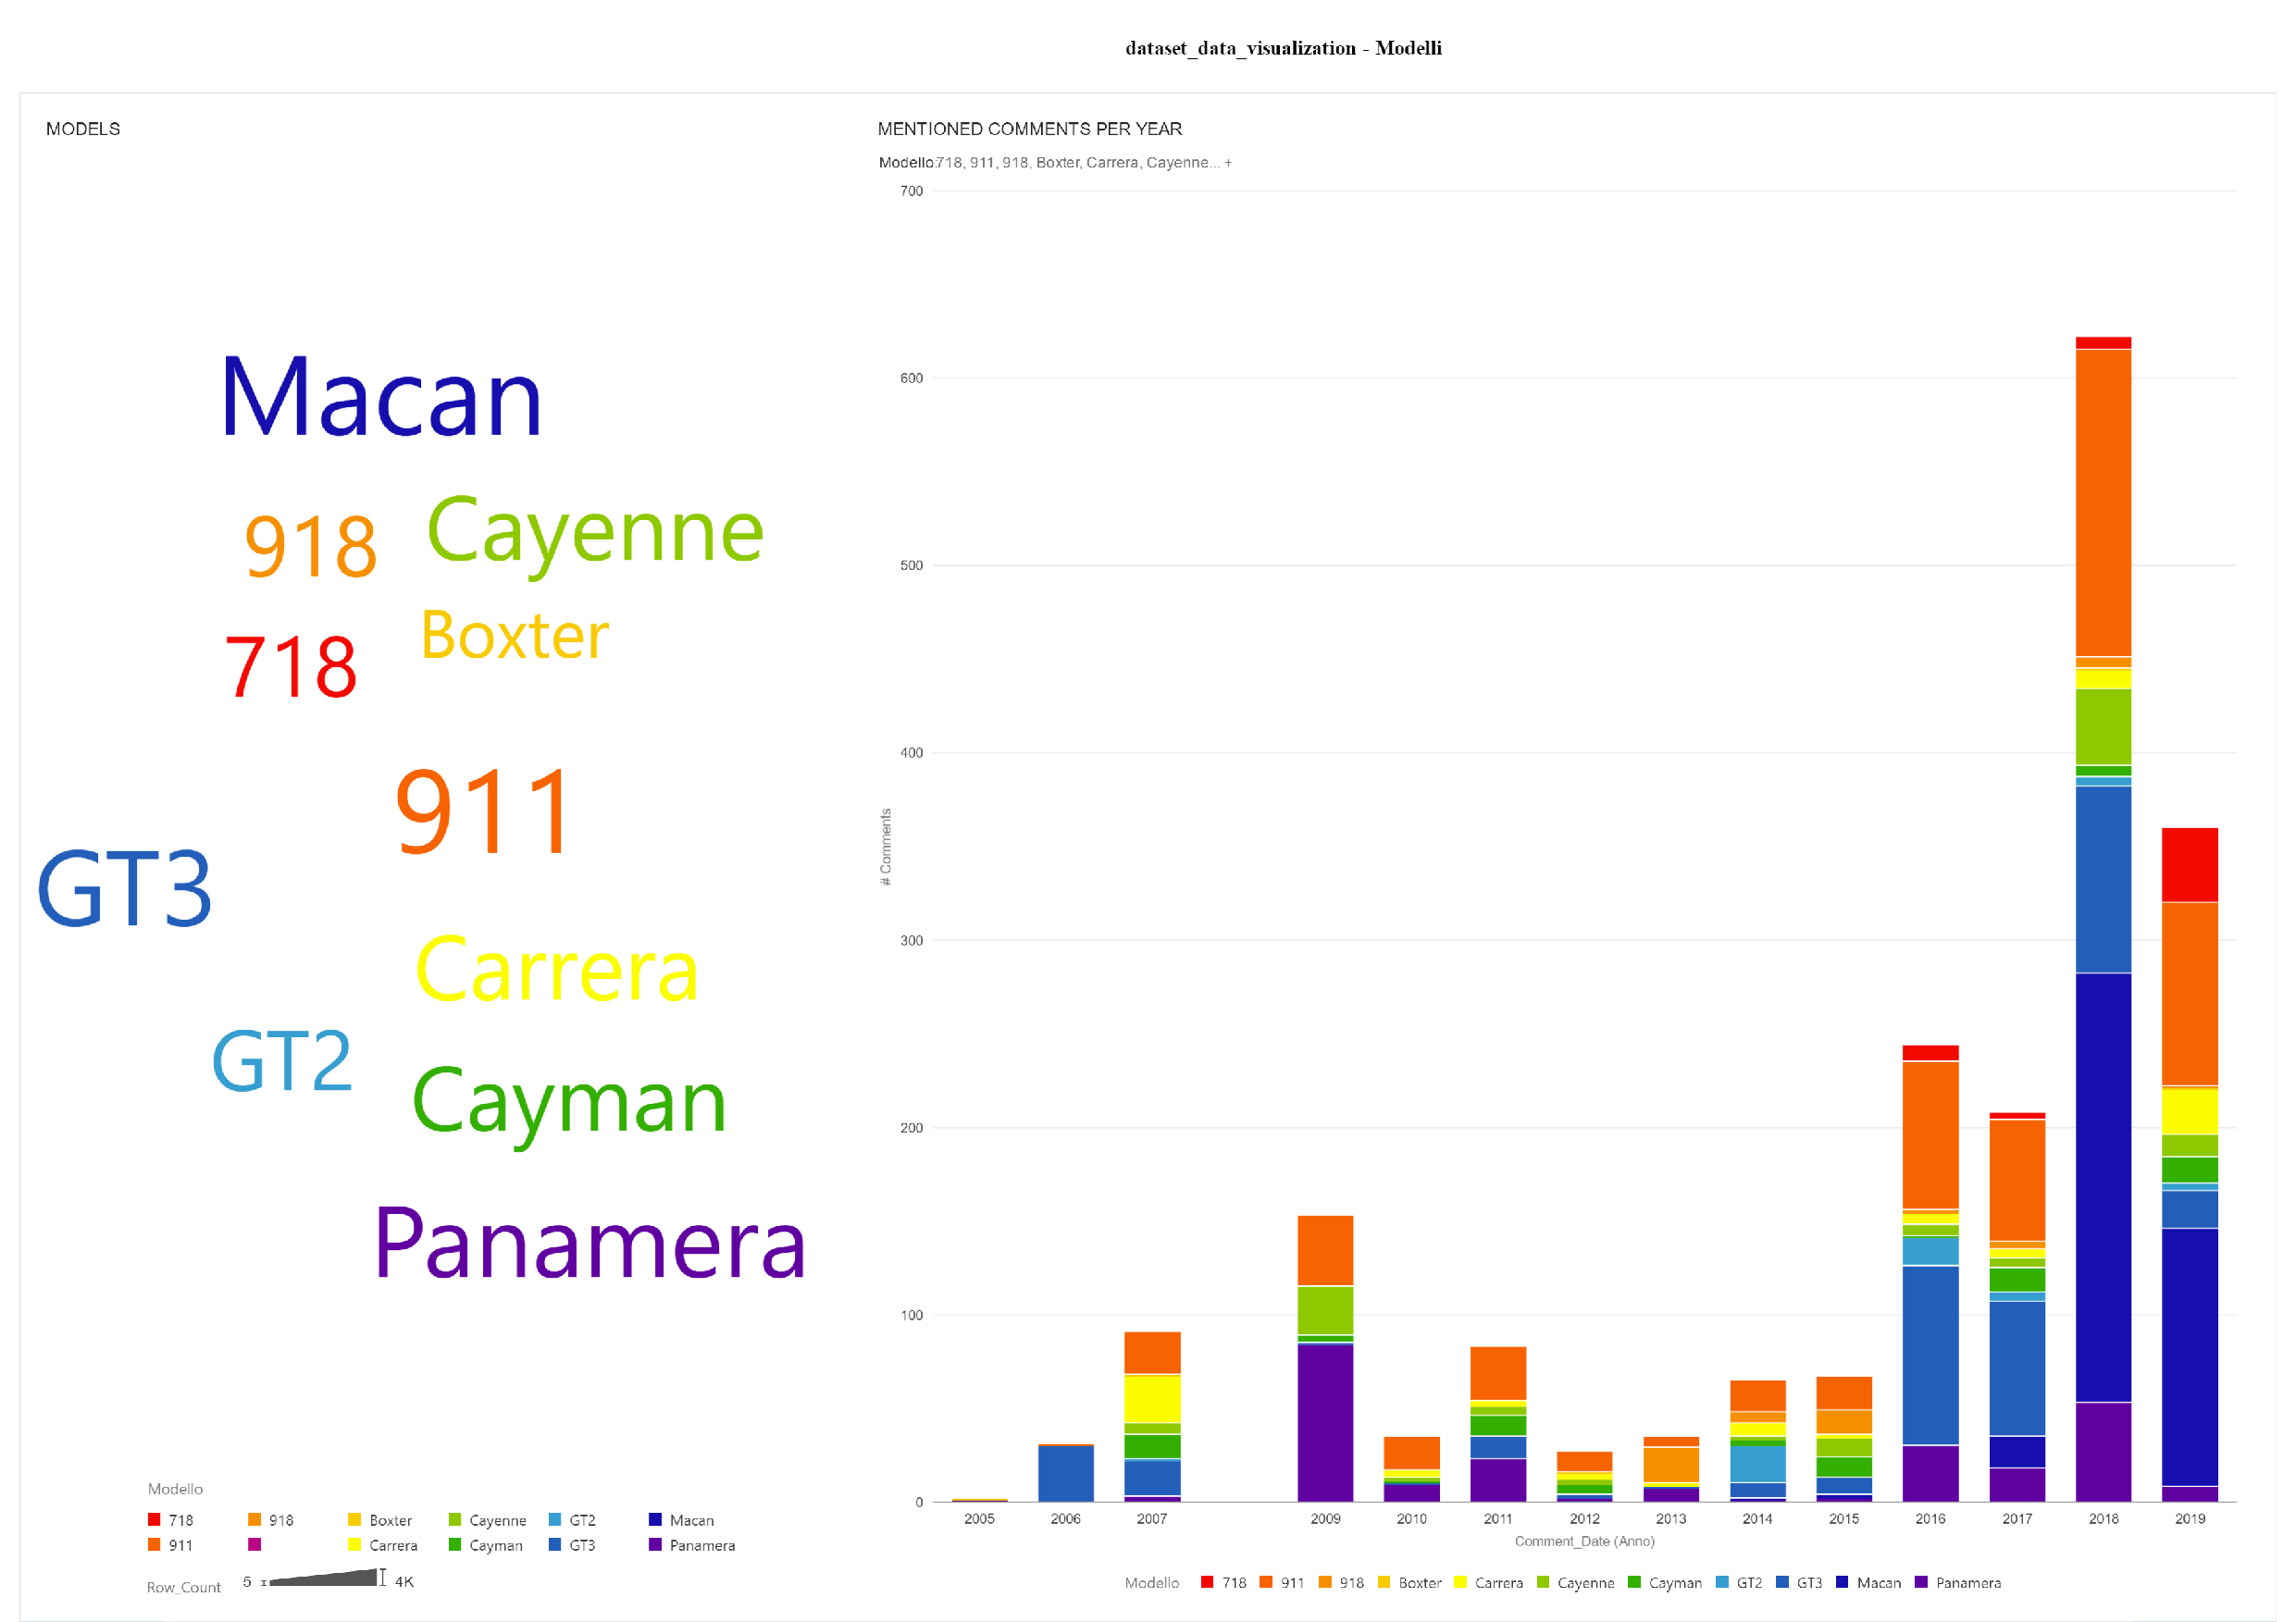
\includegraphics[width=\textwidth]{figures/odv_export/dataset_data_visualization_13.pdf}
	\caption{Most discussed models.}
	\label{fig:models}
\end{figure}

As expected, the most commonly discussed models remain almost the same over time, for instance the 911 and the Panamera, with some growing in the last years on the Macan.
\\\\\\
With Oracle Data Visualization it is also possible to inspect comments' details, which is very useful to verify the reliability of the classification, and for marketing purposes, to get customers' critics in order to make eventual brand enhancement's choices.


